\chapter{Design}

V kapitole design popíšeme návrh realizace požadavků, které jsme popsali v kapitole analýza.

\section{Architektura aplikace}

Jako implementační jazyk jsme zvolili jazyk Java.

\subsection{Serverová část}

% TODO definice Cloudu
Serverová část aplikace poběží na serverech v Cloudu, to nám umožní efektivní správu prostředků, možnost trvalé expanze a škálovatelnost aplikace.
Pro volbu konkrétního poskytovatele jsme měli (v době zahájení práce) na výběr z:
\begin{itemize}
	\item Amazon EC2
	\item Google AppEngine
\end{itemize}

Jelikož jsme měli již zkušenost s druhým zmíněným a jeho architektura a API nám byla známá, zvolili jsme jej.

\subsubsection{Platforma Google AppEngine}

% TODO definice VPS
Google AppEngine je platforma pro vývoj a hostování webových aplikací psaných v jednom z několika podporovaných jazyků.
Poskytovatel účtuje jen prostředky skutečně využité, tím se liší od běžných VPS.
Platforma umožnuje automatické škálování výkonu podle aktuální potřeby aplikace.
Samotný výběr poskytovatele nám umožňuje splnit výkonostní požadavky.

AppEngine je platforma, která poskytuje několik spolu provázaných rozhraní.
Pro naši aplikaci jsou důležité především:
\begin{itemize}
	\item Datastore -- databáze pro uložení všech dat, jak sdílených, tak i dedikovaných jednotlivým uživatelům.
		Specifikem této databáze je, že formálně nemá schéma a má jen velice omezené možnosti dotazování na úkor výkonu.
		Mezi největší omezení patří nemožnost jakýchkoli spojení tabulek, veškeré filtry použité v dotazu mohou jen porovnávat hodnotu atributu s konstantou; toto omezení nutně ovlivnilo návrh entit a implementaci tříd.
		Dalším omezením je nutnost existence perfektního indexu pro každý dotaz, který se kdy bude provádět; neexistence indexu způsobí běhovou chybu.
		Na druhou stranu, nutnost zaindexování všech dotazů umožňuje extrémní rychlost databáze; každý dotaz se provádí ve dvou krocích:
		1. nalezení prvního výsledku v indexu; 2. výpis nalezeného záznamu a všech následujících, dokud záznam vyhovuje všem filtrům.
		Existují ještě další omezení, které nás příliš netrápí, například, že dotaz může vrátit neaktuální výsledky.
	\item Task Queue -- fronta úloh, skrze kterou projdou všechny úlohy.
		Fronta se stará o pravidelné spouštění úloh s pevnou frekvencí; to zajišťuje, že při kontrole zdrojů nedojde k většímu zatížení serveru.
		Kontrola každého zdroje je jedna úloha a fronta úloh se stará o to, aby bylo spuštěno jen určité množství úloh zároveň.
	\item Users -- ověřování uživatelů; aplikace přebírá údaje o aktuálně přihlášeném uživateli při každém požadavku.
		Nemusíme tedy řešit celou infrastrukturu kolem registrace, přihlašování, odhlašování, zapomenutého hesla.
	\item BlobStore a Files -- jelikož architektura serveru neumožňuje práci s filesystémem -- není známá informace o tom, na kterých serverech a kde na světě aplikace právě běží (potenciálně v několika instancích) -- posktuje server rozhraní ke své abstrakci souborů.
		My toto API použijeme k uložení a následné prezentaci zazálohovaných webových stránek článků.
\end{itemize}

\subsubsection{Úloha serverové části}

Serverová část bude mít v aplikaci následující úlohy:
\begin{itemize}
	\item uložení všech dat,
	\item poskytování dat klientům,
	\item periodický sběr nových položek kontrolou zdrojů,
	\item výpočet doporučení zdrojů klientům na základě podobnosti.
\end{itemize}

\subsubsection{Použité knihovny}

Abychom znovu nevynalézali kolo a neřešili problémy, které již jiní řešili před námi, použijeme několik knihoven, které nám zjednodušší implementaci vlatní aplikace.

\paragraph{Slim3}
% TODO link Slim3
Pro obalení nízkoúrovňového API pro přístup k databázi použijeme framework Slim3.
Slim3 zajišťuje mapování databázových bezschématických entit na reálné javové objekty.
Tento framework zároveň poskytuje objektově konzistentní rozhraní ke skládání databázových dotazů.
Tato knihovna je vyvinutá jen a pouze pro platformu AppEngine, neboť je silně závislá na Datastore API.

\paragraph{ROME}
%TODO link ROME
ROME je knihovna, která poskytuje sadu parserů a generátorů pro různé typy formátů zpravujících o novinkách na webovém zdroji.
My tuto knihovnu použijeme pro oba směry konverze, využijeme parsery při kontrole jednoho typu zdrojů a generátory při sdílení (exportu) položek.
ROME je starší knihovna, nezdá se, že by její vývoj pokračoval, nicméně je dostatečně robustní a stabilní pro naše potřeby.

\paragraph{Apache HttpComponents}
% TODO apache http components
% definice http
Apache HttpComponents je široce rozšířená kni\-hov\-na uřcená pro zajištění komunikace přes HTTP.
My ji použijeme pro stahování webových dokumentů při kontrole zdrojů všech typů (kromě manuálního).

\paragraph{JSOUP}
% TODO vysvětlit DOM
% TODO link jsoup
Knihovna jsoup umožňuje rozparsovat HTML stránku do DOM struktury a poskytuje metody na procházení a manipulaci se stromem elementů.
Knihovna zvládá zpracování i takových stránek, které nevyhovující standardům.
My knihovnu využijeme ve dvou situacích:
\begin{itemize}
	\item pro parsování webové stránky při kontrole některých typů zdrojů,
	\item pro úpravu relativních odkazů při zálohování webové stránky.
\end{itemize}

\paragraph{JScience}
% TODO link JScience
Knihovna JScience poskytuje implementaci nejrůznějších výpočetních algoritmů určených pro matematiku a fyziku.
Nás z této knihovny bude zajímat jen malá část: implementace vektorových a maticových operací, které použijeme při výpočtech doporučených zdrojů pro jednotlivé uživatele.

\paragraph{Diff Match Patch}
% TODO link diff match patch
Diff match patch je malá knihovna, která nabízí robustní algoritmy pro operace nutné při synchronizaci textu.
My využijeme jen jednu ze tří částí: porovnání dvou textů, které nám vrátí seznam rozdílů.

\subsection{Klientská část}

% TODO vysvětlit html, css, js
Klientská část naší apliakce je ta část, kterou si každý uživatel stáhne při návštěvě webové stránky aplikace.
Jelikož se aplikace spouští v internetovém prohlížeči, je omezená tímto prostředím: grafická část je tvořena jazykem HTML a CSS, výkonná část je napsána v jazyce JavaScript.
Jelikož serverová část aplikace je vytvořena v jazyce Java, zvolili jsme pro klientskou část nástroj, který umožňuje zkompilovat kód v jazyce Java do jazyku JavaScript, který je určen pro běh v prohlížeči.
Takovým nástrojem je Google Web Toolkit -- GWT; mezi jeho základní vlastnosti patří:
\begin{itemize}
	\item serverová i klientská část je psána ve stejném jazyce,
	\item společný kód pro serverovou a klientskou část se napíše jen jednou (a přeloží dvakrát),
	\item poskytuje základ pro komunikaci mezi klientskou a serverovou částí, stará se o serializaci a deserializaci požadavků,
	\item stará se o minifikaci kódu odeslaného klientovi,
	\item poskytuje hotové základní komponenty pro tvorbu uživatelského rozhraní.
\end{itemize}

\subsubsection{Úloha klientské části}

Klientská část je část aplikace, kterou uživatel ovládá pomocí prvků grafického prostředí webové stránky.
Skrze ní manipuluje se svými daty uloženými v serverové části aplikace.
Mezi nejdůležitější úkony prováděné uživatelem patří:
\begin{itemize}
	\item správa zdrojů: přidání a úprava zdroje, zastavení a obnovení sledování zdroje
	\item procházení seznamu položek, zobrazení originálu položky, přidání/odebrání štítku, zazálohování položky
	\item filtrování seznamu položek, změna kritérií filtru, správa filtrů
	\item nastavení ostatních vlastností aplikace
\end{itemize}

\subsubsection{Použité knihovny}

V klientské části aplikace použijeme jedinou knihovnu: GWT Eye Candy.
Tato knihovna nabízí kolekci ovládacich prvků do uživatelského prostředí aplikace.
My využijeme jen jediný prvek: ColorPicker pro výběr barvy štítků.

\subsection{Doplněk do prohlížeče}

% TODO link na crossrider
Využijeme služeb platformy Crossrider, která umožňuje vytvořit jediný doplněk, který bude fungovat shodně v nejrozšířenějších prohlížečích.
Podporované prohlížeče jsou:
% TODO link na FAQ 
\begin{itemize}
	\item Internet Explorer 7 a vyšší
	\item Chrome -- všechny verze
	\item Firefox -- 3.6 a vyšší
\end{itemize}

\subsubsection{Funkce doplňku}
% XXX Moc podrobně?

Doplněk slouží k přidání nové manuální položky do aplikace.
Doplněk bude mít podobu tlačítka na liště v prohlížeči; kliknutím na tlačítko se objeví vyskakovací okno s předvyplněnou adresou a titulkem aktuální stránky.
V připadě, že uživatel vybere část textu na stránce, bude jím předvyplněn popis.
Kliknutím na tlačítko \uv{Odeslat} se vytvoří v aplikaci nová manuální položka podle vyplěných údajů.

\subsubsection{Použité knihovny}

% TODO knihovny v doplňku

\section{Entity}

Entity jsou obecné struktury, se kterými aplikace pracuje.
Cílem této kapitoly je entity popsat a vysvětlit úlohu, kterou hrají v kontextu celé aplikace.
Pro přehlednost jsme entity sdružili do oblastí, jichž se týkají.

\subsection{Oblast uživatele a konfigurace}

Oblasti uživatle a konfigurace obsahuje následující entity:

\subsubsection{Uživatel}

Uživatel je reprezentace osoby, která systém používá.
Entitu uživatele přebíráme od poskytovatele serveru pomocí Users API.

\subsubsection{Konfigurační položka}

Konfigurační položka nemá nic společného s termínem položka ani entitou položka.

Jedna konfigurační položka definuje jeden parametr, který má vliv na vzhled nebo chování aplikace; lze rozlišit dva typy konfiguračních položek:
\begin{itemize}
	\item konfigurace serverové části -- závisí na ní chování serverové části,
	\item konfigurace klientské části -- závisí na ní vzhled nebo chování klientské části.
		Hodnoty položek tohoto typu mohou záviset na konkrétním uživateli, který aplikaci používá.
\end{itemize}

\subsection{Oblast zdrojů}

Tato část seskupuje všechny entity, které jsou souvisejí se zdroji položek, jejich reprezentací a zpracováním.
Nejdůležitější dvojicí entit je zdroj a uživatelský zdroj: první má význam pouze pro pravidelné kontroly exitence nových položek, druhá popisuje zdroj z pohledu uživatele.
Oblast zdrojů obsahuje tyto entity:

\subsubsection{Zdroj}
\label{sss:zdroj}

Zdroj reprezentuje každou webovou stránku nebo službu, kterou aplikace používá k získávání nových položek.
Aplikace pravidelně kontroluje změny na zdrojích; pokud zaregistruje změnu, aplikace přidá odpovídající položky.
Zdroj je abstraktní entita, od které jsou odvozeny jednotlivé typy zdrojů; obsahuje všechny informace nutné k tomu, aby zdroj mohl být periodicky kontrolován.
Typy zdrojů jsou:

\paragraph{Manuální zdroj}

Manuální zdroj patří vždy jednomu konkrétnímu uživateli.
Nereprezentuje žádnou internetovou adresu a sám o sobě neposkytuje žádné položky.
Všechny položky, které tomuto zdroji patří, přidal sám uživatel skrze jednu ze služeb k tomu určených.

\paragraph{RSS/Atom}

RSS a Atom jsou formáty XML dokumentů, které popisují novinky, ke kterým došlo za poslední dobu na webovém portálu.
Tento zdroj typicky obsahuje odkazy na články, které byly publikovány v nedávné minulosti.

\paragraph{Webový rozcestník}

Nahrazuje funkcionalitu RSS či Atom pro webové portály, které tyto kanály neposkytují.
Vychází z jednoduchého pozorování, že úvodní stránka takového portálu obsahuje seznam nejnovějších článků a že položky převzaté z RSS či Atomu by odpovídaly odkazům na této stránce.

\paragraph{Změna stránky}

Reprezentuje webovu stránku o jejíž změně obsahu chce být uživatel být informován.
Každá změna stránky způsobí vytvoření položky informující o změně.

\subsubsection{Region}

Region definuje pro typ zdroje Webový rozcestník a Změna stránky oblast stránky, která je z pohledu uživatele zajímavá.
Oblast na stránce je určena výběrem oblastí stránky, které se mají kontrolovat a oblastí, které se mají při kontrole ignorovat.
Motivací k pozitivnímu a negativnímu přístupu k jednotlivým částem je fakt, že stránky obsahují obsah, který se mění při každém dotazu (reklamy, informace o času generování stránky) nebo není zajímavý (hlavička a patička stránky, menu).

\subsubsection{Uživatelský zdroj}
\label{sss:uzivatelsky-zdroj}

Entita zdroj slouží výhradně pro účely periodické kontroly, proto zavedeme entitu uživatelský zdroj, jež realizuje vztah mezi uživateli a zdroji.
Několik uživatelů může sledovat stejný zdroj a každý uživatel většinou sleduje více zdrojů.
Tato entita uchovává vlastní nastavení každého zdroje zvlášť pro každého uživatele.
Počet aktivních uživatelských zdrojů určuje, politiku podle které bude probíhat jeho kontrola.
Pokud je v uživatelském rozhraní zmíněn pojem zdroj, je jím myšlena tato entita; entita zdroje nemá pro uživatele praktický význam.

Uživatelský zdroj obsahuje entitu štítek, která reprezentuje informaci o příslušnosti položky ke zdroji.
Více o tomto štítku a jeho funkci popíšeme v kapitole \ref{sss:stitek}.

\subsubsection{Shrnutí entit oblasti zdrojů}
\label{sss:shrnuti-zdroju}
Abstraktní entita zdroj má několik typů:
\begin{itemize}
	\item manuální zdroj,
	\item RSS/Atom zdroj,
	\item webový rozcestník,
	\item změna stránky.
\end{itemize}
Entita uživatelský zdroj není typem zdroje; uživatelský zdroj reprezentuje vazbu mezi uživatelem a zdrojem.

\subsection{Oblast položek}

Oblast položek obsahuje entity:

\subsubsection{Položka}

Položkou v aplikaci myslíme jednu adresu webové stránky, která pochází z některého ze zdrojů nebo byla přidána uživatelem manuálně.
Položka je závislá jen na zdroji, ze kterého pochází, vlastní personalizaci (přizpůsobení jednotlivým uživatelům) se zabývá entita uživatelská položka.
Každý typ zdroje poskytuje položky jiného typu:

\paragraph{Manuální položka}

Manuální položka formálně patří k manuálnímu zdroji; jediným důvodem je zajištění konzistence rozhraní všech typů položek.
Manuální položka reprezentuje libovolnou internetovou adresu spolu s titulkem a popisem.
Manuální položka vzniká jen a pouze činností uživatele, který si ji sám přidá do aplikace.
Motivací zavést manuální položku je umožnění uživateli:
\begin{itemize}
	\item přidat vlastní informaci k libovolné stránce,
	\item zazálohovat libovolnou stránku,
	\item označit si libovolnou stránku k pozdějšímu přečtení.
\end{itemize}

\paragraph{Položka typu článek}

Položka typu článek je produkována při kontrole zdrojem typu RSS/Atom.
Každému záznamu v XML dokumentu odpovídá jedna položka vytvořená v aplikaci při kontrole zdroje.
Titulek a popis přebíráme spolu s dalšími informacemi přímo z RSS/Atom dokumentu.
Položka typu článek může poskytovat více informací než jiné typy položek: jedná se především o jméno autora článku a datum publikace.
Obecně tyto informace nejsou jednoduše zjistitelné v případě položek jiných typů.

\paragraph{Položka typu odkaz}

Položka typu odkaz pochází ze zdroje typu webový rozcestník.
Každému nalezenému odkazu na webové stránce (uvnitř regionem omezené oblasti) odpovídá přavě jediná položka.
Titulek resp. popis přebíráme z textu odkazu reps. textu nejbližšího okolí odkazu.

\paragraph{Položka typu změna stránky}

Položka typu změna stránky pochází ze zdroje typu změna stránky.
Při kontrole stránky (na kterou se odkázuje zdroj) se porovnává její textový obsah s verzí, kterou jsme si uložili při předchozí kontrole.
Pokud je nalezena změna, aplikace vytvoří novou položku, která bude obsahovat popis změn stránky.

\bigskip{}

Položka je závislá jen na zdroji, ze kterého pochází; stejně jako v oblasti zdrojů existuje dvojice: zdroj -- uživatelský zdroj, existuje i entita uživatelská položka.

\subsubsection{Uživatelská položka}

Entita položka obsahuje jen obecné -- na uživateli nezávislé atributy, které jsou sdíleny všemi uživateli.
Jsou jimi například: titulek, obsah, zdroj, ze kterého pochází, datum a čas přidání.
Aby mohl každý uživatel mít položku ve vlastním stavu, s vlastními štítky, zavedeme entitu uživatelská položka.
Tato entita uchovává nastavení vlastní každému uživateli, včetně zálohy, pokud byla vytvořena.

Pokud je v uživatelském rozhraní zmíněn pojem položka, je jím myšlena tato entita; entita položka nemá pro uživatele praktický význam.

\bigskip{}

Na obrázku \ref{fig:source-item} je zobrazen vztah nejdůležitějších entit z oblastí zdrojů a položek.

\begin{figure}
    \centering
    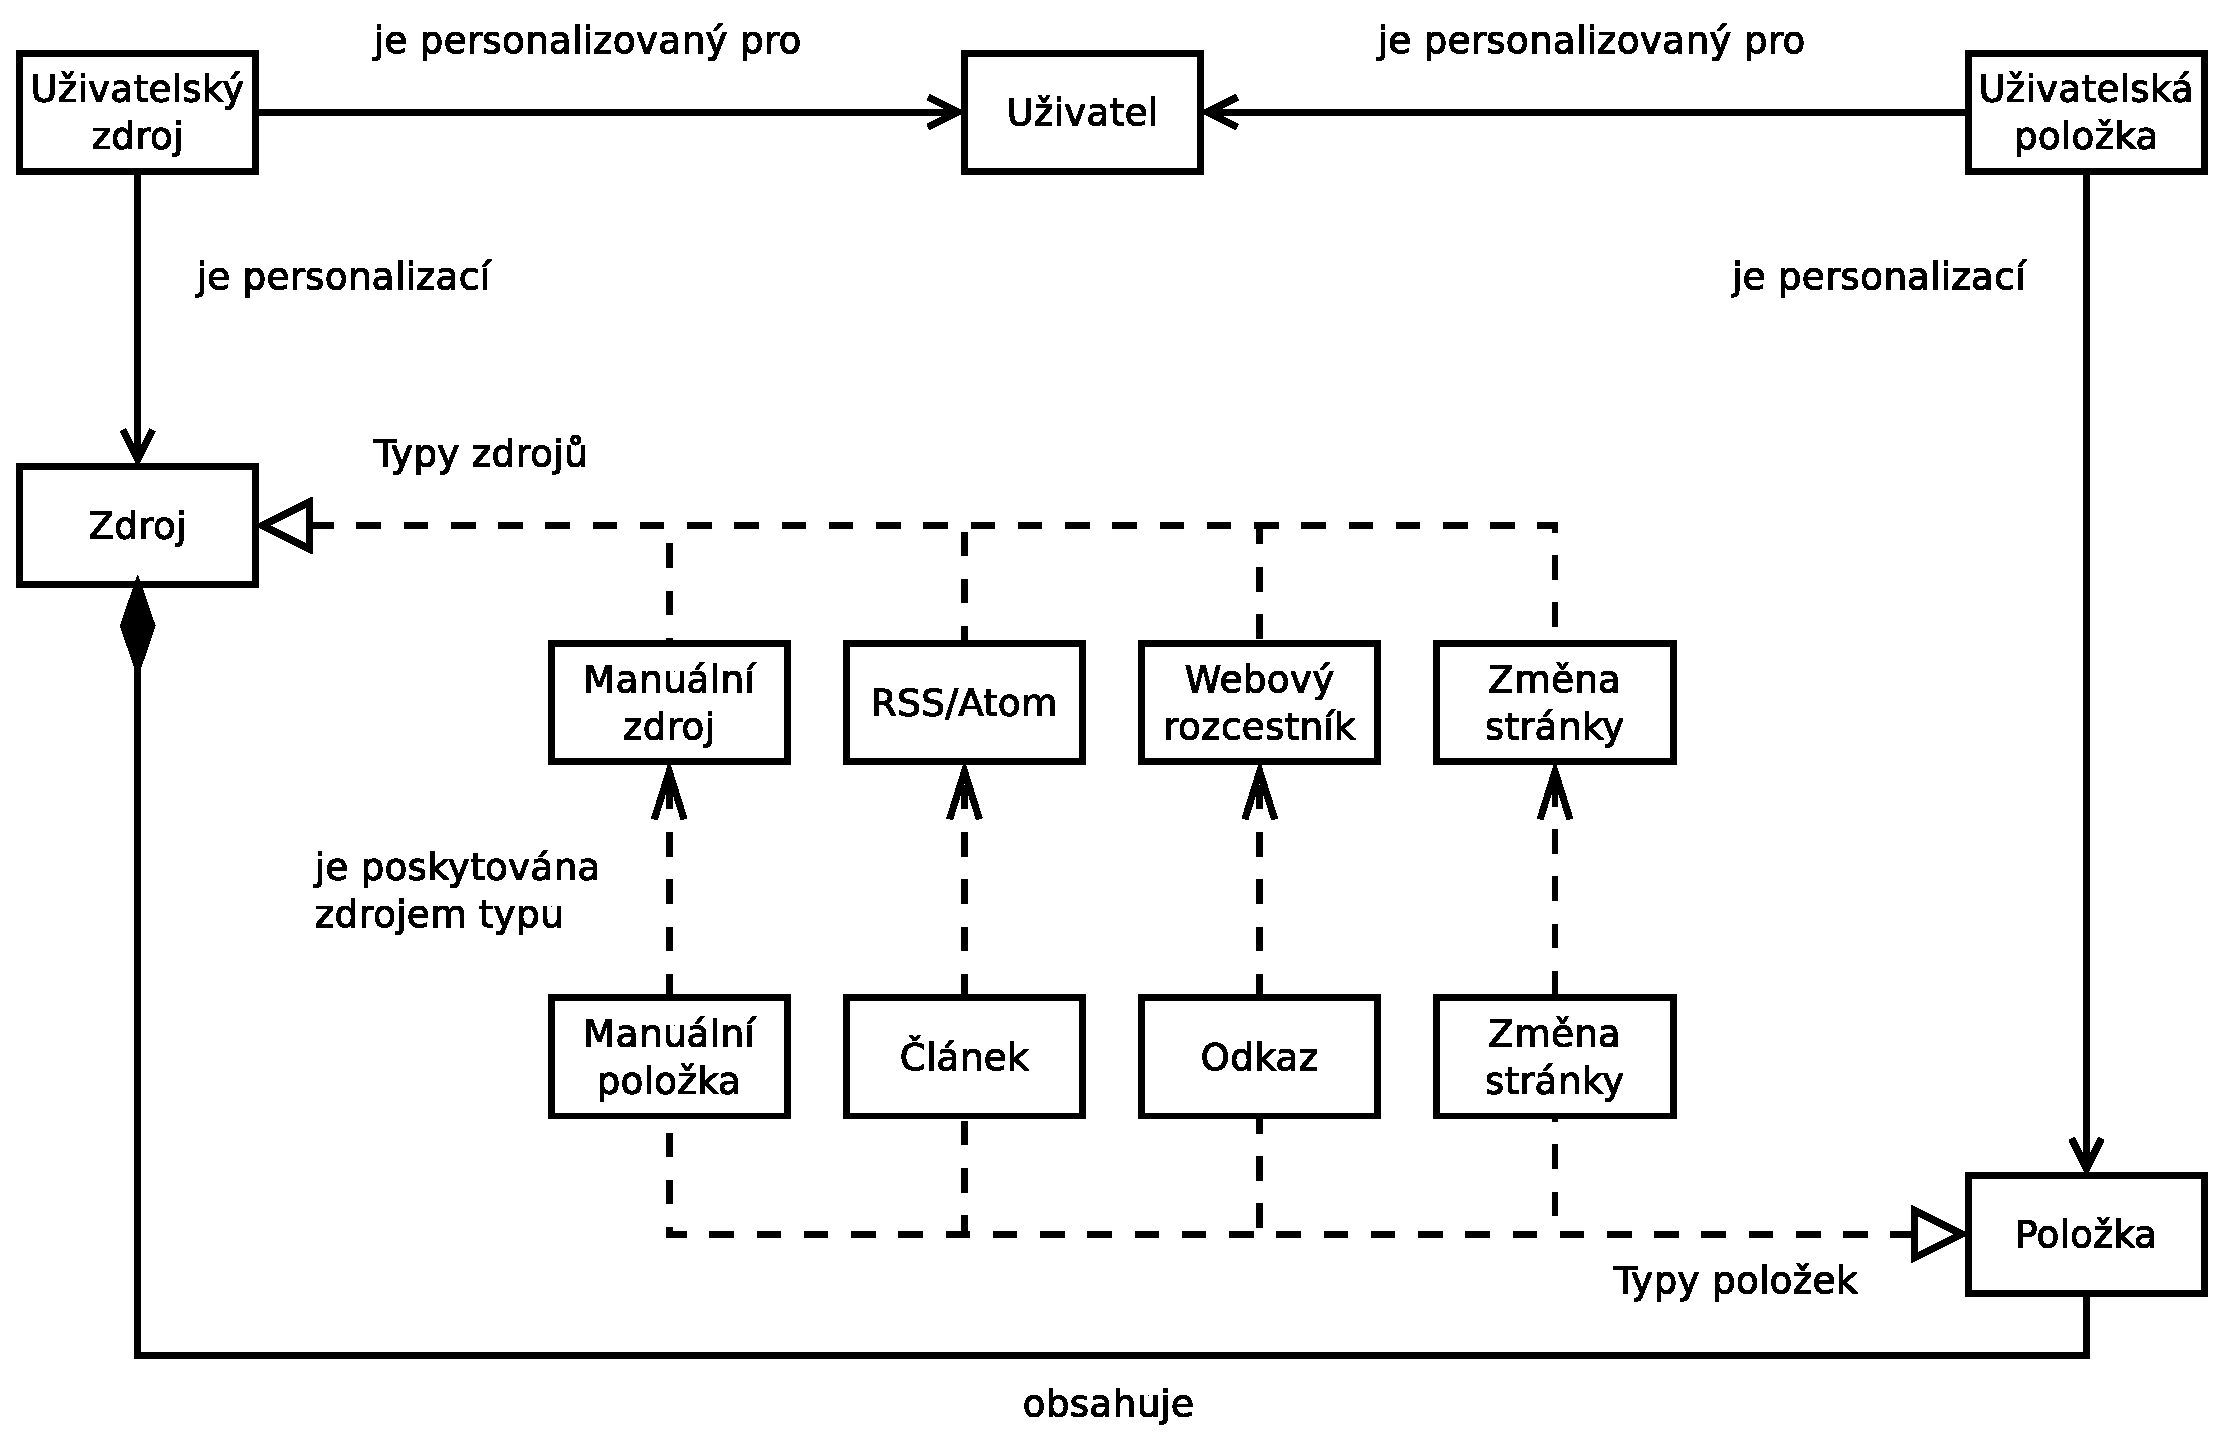
\includegraphics[width=12cm]{img/zdroje-polozky.eps}
    \caption{Vztahy mezi uživatelem, zdroji a položkami}
    \label{fig:source-item}
\end{figure}

\subsection{Oblast štítků}

Oblast štítků obsahuje entity:

\subsubsection{Seznam položek}
Než zavedeme entity této oblasti, zadefinujeme pojem seznam položek.

Seznam (uživatelských) položek je podle času vzestupně či sestupně uspořádaný seznam všech uživatelských položek, které vyhovují všem kritériům, které jsou uživatelem na seznam kladeny.
Seznam položek je výsledkem dotazu, neexistuje dokud není dotaz proveden.

Termín seznam položek používáme také pro komponentu grafického prostředí, která zobrazuje uživatelké položky, které jsou součástí seznamu položek, výsledku dotazu.

\subsubsection{Štítek}
\label{sss:stitek}

Štítek reprezentuje informaci, kterou může uživatel přidat ke své uživatelské položce.
Štítek má svého vlastníka, uživatele, který jej vytvořil; tento štítek není dostupný jiným uživatelům.
Štítek má několik úloh:
\begin{itemize}
	\item tvoří poznámku u uživatelské položky,
	\item lze filtrovat uživatelské položky mající přiřazený konkrétní štítek,
	\item přiřazením vhodného štítku k uživatelské položkce se provede záloha webové stránky položky.
\end{itemize}

Abychom zajistili jednoduché používání štítků, zavedli jsme následující dvě omezení:
\begin{itemize}
	\item Název štítku nesmí obsahovat bílé znaky a znak \$.
		Bílé znaky na okrajích názvu se oříznou, bílé znaky uvnitř a znak \$ způsobí chybu při vytváření/přiřazování štítku.
		Toto omezení vynucuje výstižná jednoslovná pojmenování štítků.
	\item Název štítku nelze později změnit.
		Toto omezení umožňuje využít název štítku jako část jeho klíče.
\end{itemize}

V aplikaci existují dva typy štítků:
\begin{enumerate}
	\item uživatelský štítek -- štítek, který vytvořil uživatel, je přiřazovaný uživatelem a je zobrazovaný v seznamu položek,
	\item zdrojový štítek -- štítek reprezentující uživatelský zdroj -- tento typ štítku není spravován uživatelem, nemůže jej ani vytvořit ani přiřadit, nezobrazuje se v seznamu položek.
\end{enumerate}

\paragraph{Seznam štítků u uživatelských zdrojů}
Uživatel má možnost u svého uživatelského zdroje uvést seznam štítků, které mají být automaticky přidány ke každé uživatelské položce, která patří danému uživatelskému zdroji.
V případě, že zdroj je typu manuální zdroj, nebudou štítky přidány k uživatelské položce automaticky, ale budou jen uživateli nabídnuty přednostně.

Každý uživatelský zdroj obsahuje právě jeden zdrojový štítek; tento štítek zároveň patří právě jednomu uživatelskému zdroji a je vždy součástí zmíněného seznamu štítků.

Můžeme říct, že existuje dvojí vazba mezi uživatelským zdrojem a jeho uživatelskými položkami:
\begin{enumerate}
	\item přímá vazba uživatelské položky na uživatelský zdroj;
	\item nepřímá vazba přes společný zdrojový štítek.
		Tuto vazbu využijeme dále při popisu entity seznamový filtr.
\end{enumerate}

\subsubsection{Seznamový filtr}

Seznamový filtr popisuje kritéria a způsob řazení seznamu položek.
Řazení je vždy buď sestupně či vzestupně podle času přidání uživatelské položky.
Možná kritéria jsou následujících typů:
\begin{itemize}
	\item přečtená/nepřečtená uživatelská položka,
	\item nejstarší/nejnovější datum přídání uživatelské položky,
	\item filtr tvořený predikáty: \uv{Uživatelská položka $X$ má přiřazený štítek $Y$}
\end{itemize}

Poslední uvedené kritérium je zásadní pro funkčnost celé aplikace a všech seznamů položek:
\begin{itemize}
	\item seznam všech položek -- filtr je prázdný
	\item položky nějakého uživatelského zdroje -- filtr obsahuje štítek patřící uživatelskému zdroji
	\item složitější filtry, například seznam položek ze zdroje $X$ nebo položek obsahující zároveň štítek $a$ a $b$:
		\verb|lsrc$X OR lusr$a AND lusr$b|
\end{itemize}

\paragraph{Typy filtrů}
V rámci aplikace rozjišujeme tři typy seznamových filtrů.
\begin{itemize}
	\item obyčejný seznamový filtr -- seznamový filtr, který si uživatel uložil a kdykoli si může zobrazit seznam položek, které mu vyhovují,
	\item exportovaný seznamový filtr -- chová se shodně jako obyčejný seznamový filtr; umožňuje navíc zobrazit seznam položek jako RSS či Atom dokument komukoli mimo naši aplikaci,
	\item ad-hoc seznamový filtr -- slouží pro okamžitou navigaci mezi různými seznamy položek v aplikaci, není trvale uložený.
		Ad-hoc seznamovým filtrem je například realizován seznam položek zobrazený po kliknutí na libovolný štítek.
\end{itemize}

\subsection{Oblast klávesových zkratek}

V aplikaci existuje jediná entita, která popisuje klávesové zkratky.

\subsubsection{Klávesová zkratka}

Klávesová zkratka definuje chování aplikace, které nastane při stisku klávesy či kláves.
Každý uživatel si může definovat svou vlastní sadu klávesových zkratek.
Rozlišujeme tři různé typy klávesových zkratek:
\begin{itemize}
	\item zkratky, které přiřazují či odebírají štítky uživatelským položkám.
		Klávesová zkratka má vazbu na štítek, který se má k uživatelské položce přidat, pokud přiřazen není, či odebrat, pokud je již přiřazen.
	\item zkratky, které zobrazují seznam položek.
		Klávesová zkratka má vazbu na seznamový filtr, který se má použít pro zobrazení seznamu položek.
	\item zkratky, které vykonávají jednu z mnoha podporovaných akcí.
		Takovou akcí může být přechod na následující položku, zrušení aktuálního filtru či zobrazení originální stránky položky.
\end{itemize}

\section{Procesy}

Na tomto místě popíšeme procesy, které manipulují s entitami.
Z popsaných procesů je zřejmé, jak jsou jimi realizovány jednotlivé funkční požadavky na aplikaci.

\subsection{Zdroje}

Entity oblasti zdrojů jsme shrnuli v kapitole \ref{sss:shrnuti-zdroju}.
Po přihlášení si uživatel může vytvořit své vlastní zdroje:
\begin{enumerate}
	\item zjistí se, zda takový zdroj už existuje (URL a typ zdroje),
	\item pokud neexistuje vytvoří se nový zdroj příslušného typu,
	\item vytvoří se uživatelský zdroj, který propojí zdroj s uživatelem.
\end{enumerate}

Uživatel nebude moci vytvořit zdroj typu manuální zdroj; manuální zdroj se vytvoří automaticky při prvním přihlášení.
Při každém přihlášení se zkontroluje, zda existuje; pokud neexistuje, vytvoří se výše uvedeným postupem.

Odstranění zdroje není možné z důvodu, že mohou existovat položky, které jsou na něj navázané.
Uživatel může zrušit sledování zdroje změnou vlastnosti uživatelského zdroje; sledování zdroje může uživatel obnovit.
Pokud bylo u zdroje zrušeno sledování, nebudou se nadále vytvářet uživatelské položky pro tento uživatelský zdroj.
V případě, že neexistuje aktivní uživatelský zdroj pro zdroj, nebude se provádět jeho kontrola.
K tomu může dojít dvěma způsoby:
\begin{itemize}
	\item buď uživatel zrušil sledování zdroje,
	\item nebo během vytváření uživatelského zdroje došlo k chybě.
\end{itemize}

\subsection{Položky}

Aplikace pravidelně provádí kontrolu zdrojů; stáhne z internetu dokument odpovídající adreses zdroje a zpracuje jej.
Pokud se při kontrole zdroje zjistí, že záznam ještě v aplikaci neexistuje, bude vytvořen.
\begin{enumerate}
	\item Vytvoří se položka podle typu zdroje,
	\item vytáhne se z databáze seznam všech aktivních uživatelských zdrojů pro daný zdroj,
	\item vytvoří se nová uživatelská položka pro každý aktivní uživatelský zdroj.
\end{enumerate}

Uživatel může přidat do aplikace webovou stránku jako novou položku.
V případě, že uživatel přidává položku manuálně:
\begin{enumerate}
	\item nalezne se uživatelský zdroj odpovídající uživatelovu manuálnímu zdroji,
	\item vytvoří se manuální položka pro manuální zdroj nalezeného uživatelského zdroje,
	\item vytvoří se uživatelská položka pro nalezený uživatelský zdroj.
\end{enumerate}

\subsection{Seznamy položek}

Seznam položek je definován seznamovým filtrem -- několika kritérii, kterým musí každá položka vyhovět.
Ad-hoc seznamový filtr vzniká v aplikaci přirozeně akcemi uživatele, je jím realizován například výpis položek uživatelského zdroje.
Uživatel může zobrazit seznam položek na základě svého ad-hoc seznamového filtru; takový seznamový filtr může dále pojmenovat a uložit.
Uživatel si může zadefinovat libovolné množství vlastních seznamových filtrů, přeneseně i seznamů položek.
Seznamový filtr může dále měnit, případně odstranit.

\subsection{Štítky}

Uživatel má možnost přidat k položce dodatečnou informaci prostřednictvím štítku; přidání štítku může probíhat i polo-automaticky (klávesovou zkratkou) či plně automaticky (uvedením štítku do seznamu automaticky přidávaných štítku v uživatelském zdroji).

Uživatel může na několika místech vybrat štítek ze seznamu existujících štítků, případně vytvořit nový, pokud žádaný štítek ještě neexistuje.
Štítek lze odstranit, za předpokladu, že není nikde v aplikaci použit: položkou, seznamovým filtrem, či klávesovou zkratkou.

Pokud má štítek nastavenou vlastnost zálohování, jeho přiřazení uživatelské položce způsobí zazálohování webové stránky položky:
\begin{enumerate}
	\item stáhne se webová stránka položky,
	\item veškeré relativní odkazy na stránce se nahradí za absolutní,
	\item uloží se soubor stránky do úložiště a zapíše klíč do uživatelské položky.
\end{enumerate}

\subsection{Klávesové zkratky}

Uživatel si může přiřadit klávesové zkratky k nejběžnějším úkonům.
Klávesová zkratku vytvoří uvedením klávesy či kombinace kláves, které spustí akci, ke které je klávesová zkratka přidána.
Uživatel může klávesovou zkratku odebrat smazáním kombinace kláves, které ji spouští.

Poté, co je klávesová zkratka definována, kdykoli uživatel stiskne příslušnou kombinaci kláves, spustí se příslušná akce.
Některé akce mohou být závislé na kontextu, ve kterém se uživatel nachází; takovými zkratkami jsou především klávesové zkratky manipulující s aktuálně vybranou uživatelskou položkou v seznamu položek.
